	\begin{figure}[h]
	\centering
		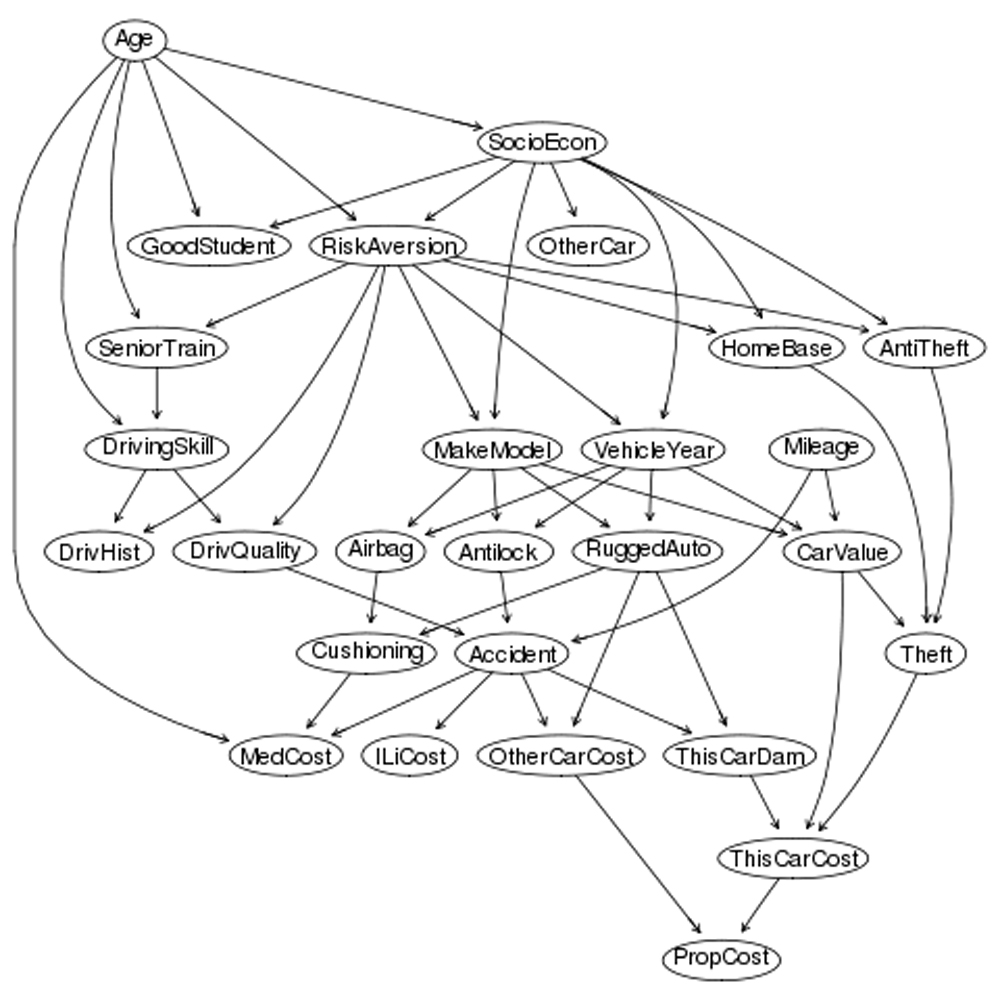
\includegraphics[height=200pt]{images/Real_Insurance}
		\caption{Bayesian network model of Insurance Evaluation Network Data Set}
	\end{figure}	

\begin{description}
	\item[Description] Insurance is a network for evaluating car insurance risks.

	\item[Number of nodes] 27
	
	\item[Number of arcs] 52
	
	\item[Number of parameters] 984
\end{description}

Binder J. \emph{et al.} (1997) motivate this example. This network for estimating the expected claim costs for a car insurance policyholder.

\begin{table}[p]																										
\centering	\caption{Comparison of scores and correct arcs via Insurance data set}	\tiny																						
{\tabcolsep=0.01in																										
\begin{tabular}{cc||cc|cc|cc||cc|cc|cc|cc}																										
\hline																										
&	&	\multicolumn{14}{c}{Insurance	(Num	of	Nodes	=	27)}\tabularnewline																			
\hline																										
\multicolumn{2}{c||}{Sample	Size}	&	\multicolumn{2}{c|}{1000}	&	\multicolumn{2}{c|}{5000}	&	\multicolumn{2}{c||}{10000}	&	&	&	\multicolumn{2}{c|}{1000}	&	\multicolumn{2}{c|}{5000}	&	\multicolumn{2}{c}{10000}\tabularnewline											
\hline																										
&	&	Sum.	&	Std.Dev.	&	Sum.	&	Std.Dev.	&	Sum.	&	Std.Dev.	&	&	&	Sum.	&	Std.Dev.	&	Sum.	&	Std.Dev.	&	Sum.	&	Std.Dev.\tabularnewline
\hline																										
\hline																										
\multirow{4}{*}{BDe} & HC &	-1427953 & 	113.01 & 	-6730331 & 	189.16 & 	-13298470 & 	246.4 & 	\multirow{4}{*}{C} & HC &	1864 & 	1.57 & 	2226 & 	0.85 & 	2414 & 	0.4\tabularnewline													
& TABU &	-1422716 & 	120.52 & 	-6708058 & 	190.97 & 	-13294810 & 	244.2 & 	& TABU &	1961 & 	1.98 & 	2543 & 	0.79 & 	2826 & 	0.68\tabularnewline													
& MMHC &	-1644392 & 	548.92 & 	-7281377 & 	826.67 & 	-14112976 & 	1680.81 & 	& MMHC &	1146 & 	1.82 & 	1457 & 	1.17 & 	1731 & 	1.88\tabularnewline													
& RSMAX2 &	-1735658 & 	397.81 & 	-8293044 & 	1714.16 & 	-16408869 & 	2342.35 & 	& RSMAX2 &	862 & 	1.42 & 	977 & 	1.77 & 	848 & 	0.61\tabularnewline													
\hline																										
\multirow{4}{*}{loglik} & HC &	-1347816 & 	118.57 & 	-6603841 & 	195.33 & 	-13134593 & 	257.01 & 	\multirow{4}{*}{M} & HC &	2253 & 	1.11 & 	1738 & 	0.79 & 	1413 & 	0.53\tabularnewline													
& TABU &	-1341071 & 	128.83 & 	-6580889 & 	194.64 & 	-13143085 & 	241.01 & 	& TABU &	2155 & 	1.39 & 	1642 & 	0.77 & 	1402 & 	0.43\tabularnewline													
& MMHC &	-1590326 & 	585.75 & 	-7192400 & 	852.4 & 	-14000007 & 	1736.44 & 	& MMHC &	3526 & 	2.2 & 	2849 & 	1.34 & 	2334 & 	2.5\tabularnewline													
& RSMAX2 &	-1687201 & 	417.78 & 	-8223919 & 	1734.08 & 	-16330085 & 	2362.44 & 	& RSMAX2 &	3761 & 	1.31 & 	3497 & 	1.05 & 	3469 & 	0.77\tabularnewline													
\hline																										
\multirow{4}{*}{AIC} & HC &	-1383888 & 	112.68 & 	-6652052 & 	190.99 & 	-13198494 & 	248.77 & 	\multirow{4}{*}{WO} & HC &	1083 & 	1.16 & 	1236 & 	0.73 & 	1373 & 	0.49\tabularnewline													
& TABU &	-1378131 & 	120.12 & 	-6629457 & 	191.37 & 	-13197529 & 	243.3 & 	& TABU &	1084 & 	1.56 & 	1015 & 	0.72 & 	972 & 	0.55\tabularnewline													
& MMHC &	-1607916 & 	566.08 & 	-7218618 & 	841.94 & 	-14033715 & 	1714.51 & 	& MMHC &	528 & 	1.39 & 	894 & 	0.76 & 	1135 & 	0.76\tabularnewline													
& RSMAX2 &	-1701145 & 	409.22 & 	-8241628 & 	1727.25 & 	-16350189 & 	2356.64 & 	& RSMAX2 &	577 & 	0.99 & 	726 & 	1.67 & 	883 & 	1.02\tabularnewline													
\hline																										
\multirow{4}{*}{BIC} & HC &	-1472404 & 	105.57 & 	-6809152 & 	185.18 & 	-13428868 & 	242.07 & 	\multirow{4}{*}{WC} & HC &	1810 & 	2.28 & 	2096 & 	1.49 & 	2240 & 	1.58\tabularnewline													
& TABU &	-1469072 & 	108.51 & 	-6787720 & 	191.17 & 	-13393809 & 	256.04 & 	& TABU &	1756 & 	2.49 & 	1906 & 	1.52 & 	1696 & 	1.46\tabularnewline													
& MMHC &	-1651080 & 	519.05 & 	-7304052 & 	808.56 & 	-14155238 & 	1635.76 & 	& MMHC &	1098 & 	2.35 & 	1494 & 	2.45 & 	1630 & 	1.43\tabularnewline													
& RSMAX2 &	-1735362 & 	389.69 & 	-8299334 & 	1705.3 & 	-16422667 & 	2335.81 & 	& RSMAX2 &	1120 & 	2.03 & 	1220 & 	1.69 & 	1596 & 	1.56\tabularnewline													
\hline																										
\end{tabular}																										
}																										
\end{table}

	\begin{figure}[p]
	\centering
		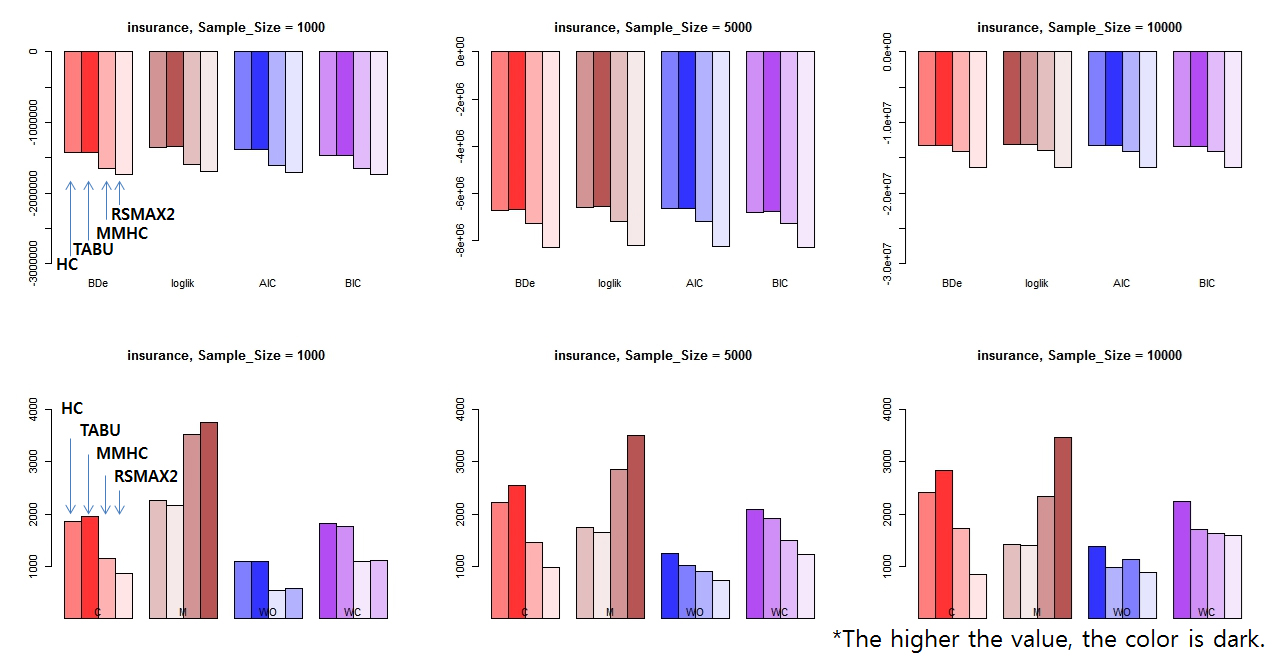
\includegraphics[height=220pt]{images/Real_2_Insurance}
		\caption{Comparison of scores and correct arcs via Insurance data set}
	\end{figure}	